\documentclass{article}

\usepackage{natbib}

\usepackage[utf8]{inputenc} % allow utf-8 input
\usepackage[T1]{fontenc}    % use 8-bit T1 fonts
\usepackage{hyperref}       % hyperlinks
\usepackage{url}            % simple URL typesetting
\usepackage{booktabs}       % professional-quality tables
\usepackage{amsfonts}       % blackboard math symbols
\usepackage{nicefrac}       % compact symbols for 1/2, etc.
\usepackage{microtype}      % microtypography

\usepackage{amsthm,amsmath,amssymb}
\usepackage{macros}
\usepackage{subcaption}
\usepackage[textfont=small, labelfont=small]{caption}
\usepackage{graphicx}
\DeclareGraphicsExtensions{.pdf,.png,.jpg,.eps}

\usepackage{algorithm}
\usepackage{algorithmic}

\usepackage[color=yellow]{todonotes}
\usepackage{booktabs}
\usepackage[inline]{enumitem}
\usepackage{verbatim}

\usepackage[left=1.5in, right=1.5in, top=1.25in, bottom=1.25in]{geometry}

\usepackage{setspace}


\title{Discrete and continuous latent states of neural activity in \textit{Caenorhabditis Elegans}}

\author{Scott W. Linderman,
  David M. Blei,
  and
  Liam Paninski
  \\
  Columbia University
}

\begin{document}

\singlespacing
\maketitle

\begin{abstract}
  Recent advances in neural recording technologies have enabled
  simultaneous measurements of the majority of head ganglia neurons in
  immobilized \celegans~\citep{kato2015global}. Moreover, since some
  neurons are known to reliably indicate the onset or offset of
  particular behaviors, like ventral and dorsal turns, behavioral
  state can be decoded from the simultaneous population recordings.
  These datasets provide unique visibility into the relationship
  between neural activity and behavior.  While it seems clear that
  activity is inherently lower dimensional than the number of neurons
  due to strong correlations between cells, the nature of the latent brain state
  remains unclear. For example, is brain state better thought of as
  discrete or continuous, or perhaps a combination of the two? Does it
  obey linear or nonlinear dynamics?  We propose a generative approach
  to probing these questions. We model the neural activity as a
  \emph{switching linear dynamical system} (SLDS), with both discrete
  and continuous latent states, and conditionally linear dynamics.  We
  then analyze the posterior distribution over states implied by the
  neural recordings and find that the discrete states correspond to
  stereotypical motor sequences. In contrast to previous work, these
  states are exposed in an entirely unsupervised manner.
\end{abstract}

% Body
\onehalfspacing

\section{Introduction}
% The world as it was:
The nematode \celegans~is unique among the model organism of
neuroscience. For decades, we have known the connectome of its 302
neurons, yet a comprehensive understanding of hows its neural activity
reflects sensory processes and produces behavior still eludes
us \citep{white1986structure}. While this connectome, or wiring diagram, has provided invaluable
information about the structure of these neural circuits, the critical
missing piece has been large scale functional measurements of these
circuits in action. With the advent of optical recording technologies,
we now possess a mounting set of tools for measuring the activity of large
fractions of these neurons simultaneously. These technologies provide
exciting opportunities to probe the link between neural activity,
sensory processing, and, ultimately, behavior.

Recently, \citet{kato2015global} have harnessed these methodological
advances to study the coordinated activity of hundreds of neurons
in head-fixed \celegans. Across multiple organisms, they have found that
neural activity reliably traces out smooth trajectories in the subspace
spanned by the first three principal components.
% TODO: Figure showing these trajectories
Upon closer evaluation, they have found that different components of these
trajectories correspond to different elements of behavior, like
forward and reverse crawling, dorsal and ventral turns, etc. These
results raise a number of interesting questions: can we learn a
(potentially nonlinear) dynamical system that approximates these
low-dimensional dynamics; is there a more appropriate subspace, or
collection of subspaces, for capturing these dynamics; can we gain
statistical power by partial, noisy recordings across separate worms
and trials; and, can we segment these trajectories in an unsupervised
manner to glean further insight into the relationship between
low-dimensional state and behavior?

% Then one day:
We have developed a probabilistic framework for investigating these questions.
The findings of \citet{kato2015global} --- namely, that neural activity
is low dimensional with behavior-specific dynamics --- suggest that
these multi-neuronal recordings may be aptly modeled in terms of
a dynamic, low-dimensional latent states. Moreover, they suggest
that neural activity may be parsed into a sequence of discrete
actions, like turning or crawling forward. These two properties are
naturally combined by \emph{switching linear dynamical systems} (SLDS),
a class of probabilistic time series characterized by co-evolving
discrete and continuous latent states.  We have extended this
class of models with a hierarchical Bayesian framework that captures
many of the nuances of these whole-brain recordings. In fitting these
models to recordings from multiple \celegans, we characterize the
globally nonlinear dynamics that govern neural activity, and we
parse these recordings into an interpretable sequence of behavioral segments.

% Raising the stakes:
% Moment of truth:
% World as it is now:
The remainder of this paper is structured as follows. In Section~\ref{sec:slds}
we introduce the class of switching linear dynamical systems and provide
some insight into the latent states and model parameters. Section~\ref{sec:hslds}
develops a hierarchical extension of the SLDS to share statistical
strength by combining recordings from multiple organisms with partially
overlapping sets of observed neurons.  Then, Section~\ref{sec:results}
presents results of applying these models to a set of recordings from
five separate \celegans. We conclude with directions for further research.


\section{Switching Linear Dynamical Systems}
\label{sec:slds}

\begin{figure}[t]
\centering%
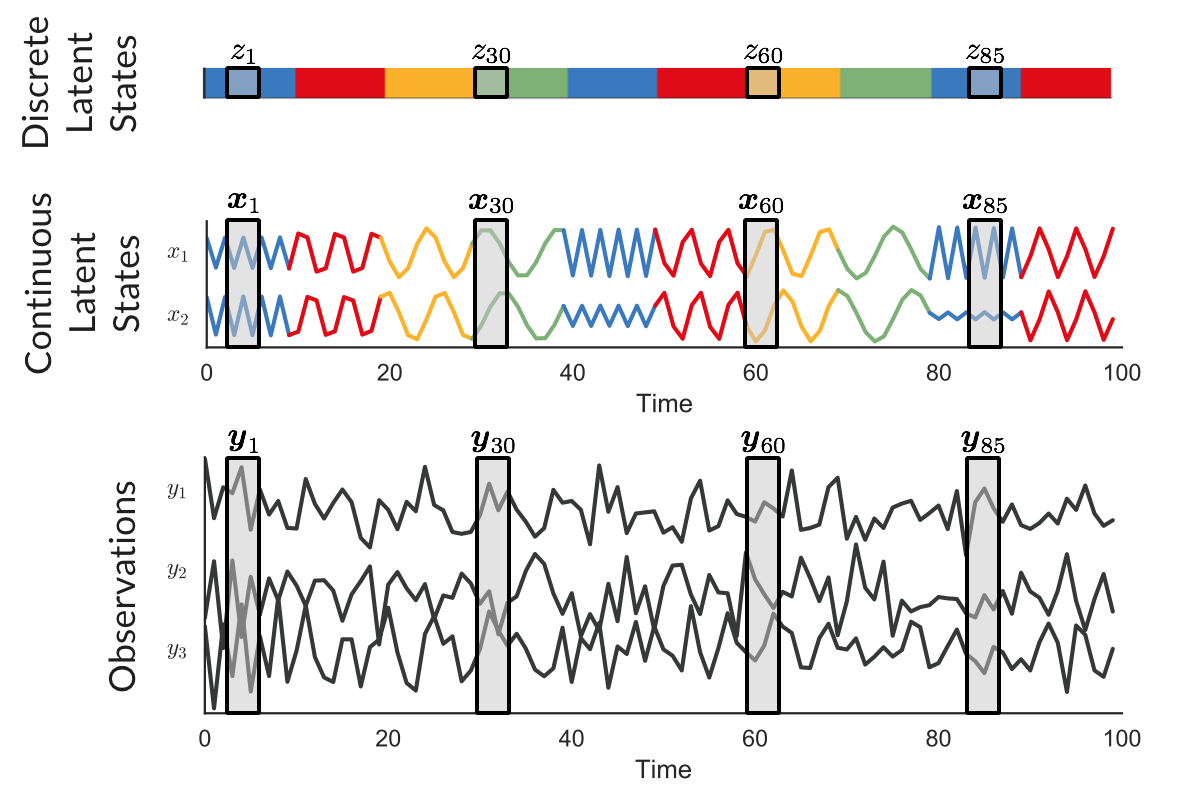
\includegraphics[width=5.5in]{slds.png} 
\caption{Simulated data from a switching linear dynamical system.  The
  population stochastically switches between discrete states,~$z_t \in
  \{1,\ldots,K\}$ (here,~$K=4$), each of which is color coded for
  visualization.  These discrete states govern the linear dynamics of
  the continuous latent state,~$\bx_t \in \reals^D$ (here,~$D=2$). For
  example, these states correspond to oscillatory dynamics with
  different frequencies. Finally, the observed signals,~$\by_t \in
  \reals^N$ (here,~$N=8$), are obtained via a linear transformation of
  the underlying, continuous state,~$\bx_t$, plus Gaussian noise. The
  correlations and dynamics in the observations are inherited from the
  dynamics of the latent states.}
\label{fig:slds_ex}
\end{figure}

The switching linear dynamical system (SLDS) is a powerful model for
stochastic time series with nonlinear dynamics \citep{ackerson1970state, chang1978state,
  hamilton1990analysis, bar1993estimation, ghahramani1996switching,
  murphy1998switching, fox2009nonparametric}, and as such, it is
particularly well suited to the analysis of whole-brain activity.
Assume the instantaneous neural activity at time~$t$ for a population
of~$N$ neurons is represented as a vector,~$\by_t \in \reals^N$. In
calcium imaging settings, the entries in this vector may be
instantaneous~$\Delta F/F$ measurements, or another signal that captures
neural activity. In this experiment, we use the smoothed time
derivative of~$\Delta F/F$. Over the course of an experiment, we
measure a sequence of vectors, which we combine into a matrix denoted
by~$\by_{1:T}$.

The SLDS model is based on the following assumptions: (i) the instantaneous
neural activity,~$\by_t$, reflects an underlying, low-dimensional
latent state; (ii) this state has a discrete component,~$z_t \in \{1, \ldots, K\}$,
and a continuous component,~$\bx_t \in \reals^D$; (iii) the continuous
latent state has linear dynamics governed by the corresponding discrete
latent state; and (iv) the observed neural activity is a linear function
of the underlying states with additive Gaussian noise.  Assumptions (i)
and (iv) are justified by the low-dimensional trajectories that
\citet{kato2015global} revealed with PCA (a linear dimensionality
reduction method). Assumptions (ii) and (iii) follow from the
trajectories naturally segment into discrete units, each with relatively
simple dynamics. 

These assumptions are formalized with the following generative model:
\begin{align}
  \label{eq:joint}
  p(\by_{1:T}, \bx_{1:T}, \bz_{1:T} \given \bTheta) &= 
  p(\bTheta)
  \prod_{t=1}^T
  p(z_t \given z_{t-1}, \bTheta) \, 
  p(\bx_t \given z_{t-1}, \bx_{t-1}, \bTheta) \, 
  p(\by_t \given z_t, \bx_t, \bTheta).
\end{align}
Beliefs about the dynamics of these latent states are encoded in the 
form of the conditional distributions for~$z_t$ and~$\bx_t$. First,
we assume the discrete states follow a Markov process,
\begin{align}
  p(z_t \given z_{t-1}, \bTheta) &\sim \bpi^{(z_{t-1})}.
\end{align}
Next, the continuous latent state is imbued with linear Gaussian dynamics,
\begin{align}
  p(\bx_t \given \bx_{t-1}, z_{t-1}, \bTheta) 
  &\sim \distNormal(\bA^{(z_{t-1})} \bx_{t-1} + \bb^{(z_{t-1})}, \bQ^{(z_{t-1})}).
\end{align}

% Figure illustrating latent dynamics
\begin{figure}[t]
\centering%
\begin{subfigure}{.24\textwidth}
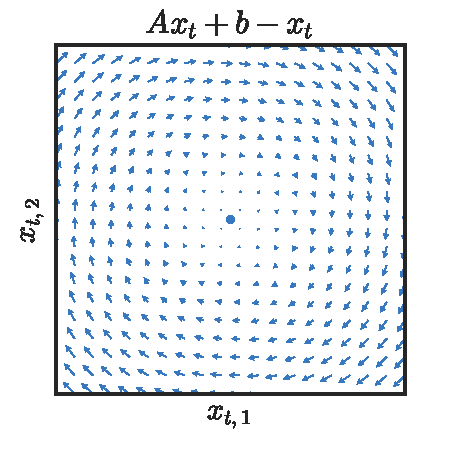
\includegraphics[width=\textwidth]{rotation_1}
\end{subfigure} 
\begin{subfigure}{.24\textwidth}
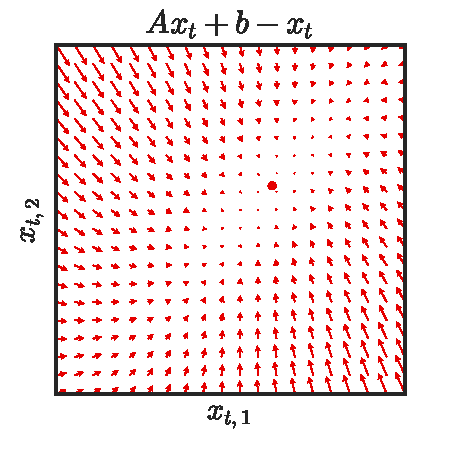
\includegraphics[width=\textwidth]{rotation_2}
\end{subfigure} 
\begin{subfigure}{.24\textwidth}
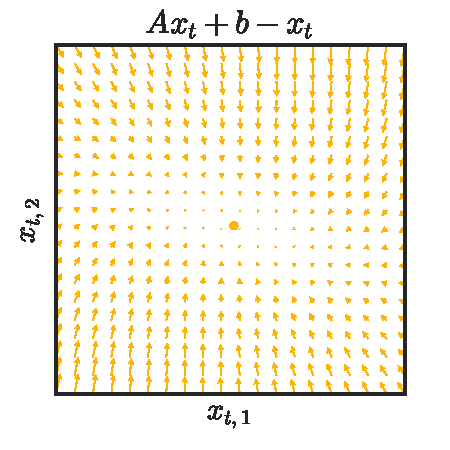
\includegraphics[width=\textwidth]{rotation_3}
\end{subfigure} 
\begin{subfigure}{.24\textwidth}
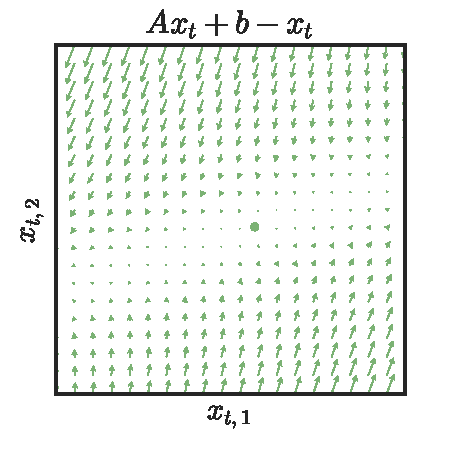
\includegraphics[width=\textwidth]{rotation_4}
\end{subfigure} 
\caption{The dynamics corresponding to discrete latent state~$k$ may
  be visualized as a vector field where the arrows point to the
  expected next state,~$\bbE[\bx_{t+1}]=\bA^{(k)}\bx_t + \bb^{(k)}$.
Here, we show the dynamics for the first and fourth discrete states 
in the synthetic example from Figure~\ref{fig:slds_ex}. The first 
discrete state is a random walk with a slight decay toward the origin;
the fourth discrete state corresponds to fast, oscillatory dynamics.}
\label{fig:slds_dynamics_ex}
\end{figure}


Finally, we impose the assumption of linear observations via the conditional
distribution,
\begin{align}
  p(\by_t \given \bx_{t}, z_{t}, \bTheta) 
  &\sim \distNormal(\bC^{(z_{t})} \bx_{t} + \bd^{(z_{t})}, \bR^{(z_t)}).
\end{align}
Thus, the parameters of the model are,
\begin{align}
  \bTheta &= \left\{ \bA^{(k)}, \bb^{(k)}, \bQ^{(k)}, \bC^{(k)}, \bd^{(k)}, \bR^{(k)}, \bpi^{(k)} \right\}_{k=1}^K .
\end{align}

Figure~\ref{fig:slds_ex} illustrates a sample from this generative model.
The observations are a sequence of vectors, in this case they are ~$N=3$ dimensional
vectors,~$\by_t$.  These states are a noisy, linear projection of an underlying
continuous latent state,~$\bx_t$, which is~$D=2$ dimensional in this case.
Here, the continuous state switches between~$K=4$ discrete regimes (four
different colors), each corresponding to different frequencies of oscillation.
The discrete state, encoded by~$z_t \in \{1, 2, 3, 4\}$ (blue, red, yellow, green),
follows a simple Markov process with transition matrix~${\bP = \{\pi^{(k)}\}_{k=1}^K}$
(not shown).

How should we interpret the these parameters? Linear dynamical
systems can essentially capture simple dynamics, like rotations, exponential
growth, and exponential decay. The stability of the system is determined
by the eigenvalues of the dynamics matrix,~$\bA^{(k)}$ --- if the eigenvalues
all have modulus less than one, the system is asymptotically stable, and
converges to a fixed point at~$(\bI - \bA^{(k)})^{-1} \bb^{(k)}$. If
the largest eigenvalue is exactly one, the system oscillates in perpetuity.
If any eigenvalue exceeds one in magnitude, the system diverges exponentially
quickly.  A variety of linear dynamical systems are illustrated in
Figure~\ref{fig:slds_dynamics_ex}. All of these systems are stable, and their
fixed points are shown as dots.

% Nonlinearity of compositional system
While the capacity of linear dynamical systems is somewhat limited,
the composition of many linear dynamical modes, as in an SLDS, yields
a highly nonlinear system. This is particularly important for modeling
neural data, which is believed to have nonlinear and often behavior-dependent
dynamics.

Given observations,~$\by_{1:T}$, our goal is to infer the discrete
latent states,~$bz_{1:T}$, and the continuous latent states,~$\bx_{1:T}$,
as well as to learn the parameters,~$\bTheta$.  We take a Bayesian
approach, specifying conjugate prior distributions for the parameters,
and using Markov chain Monte Carlo (MCMC) to estimate the posterior
distribution of the parameters and states given the observed data.
Details of this MCMC algorithm are provided in Appendix~\ref{app:mcmc}.



\section{Hierarchical Switching Linear Dynamical Systems}
\label{sec:hslds}

\begin{figure}[t]
\centering%
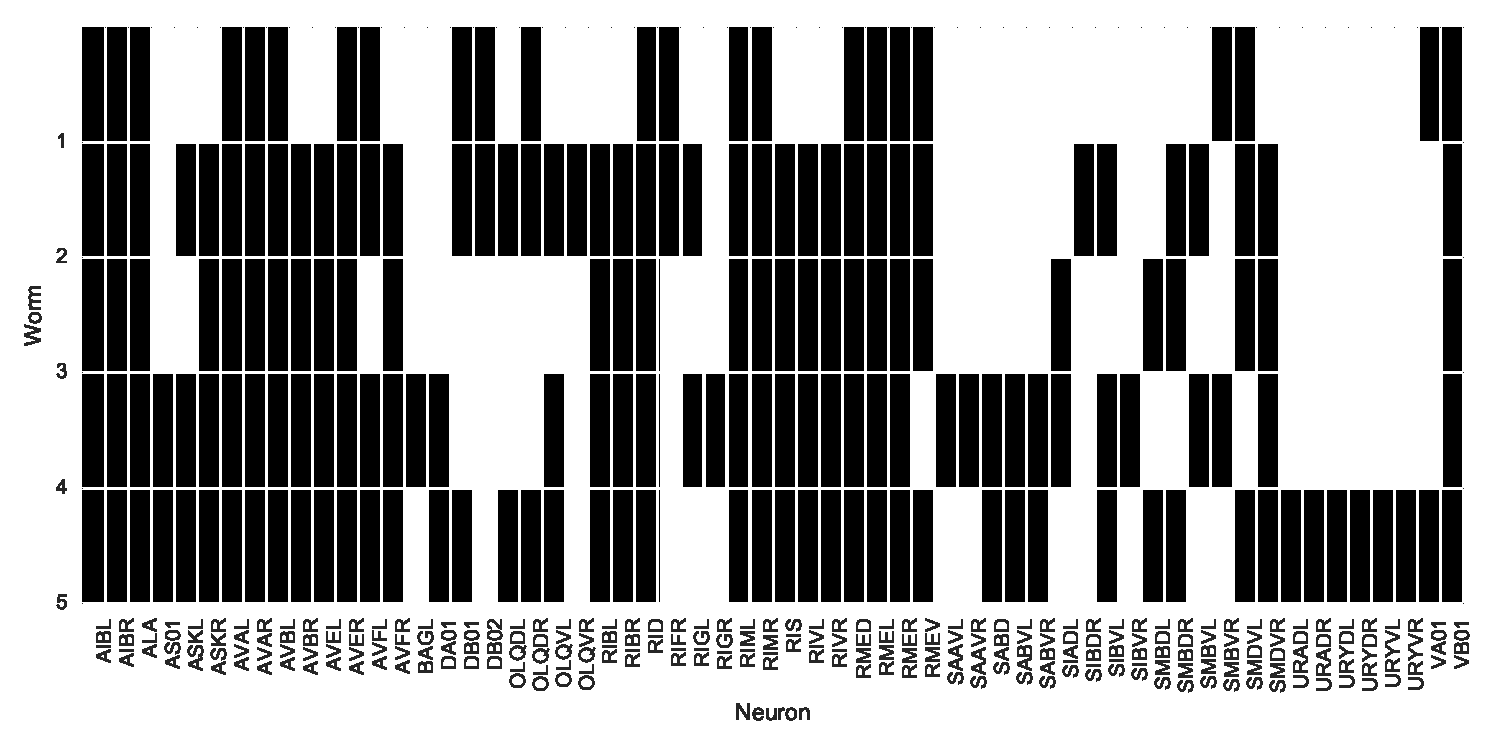
\includegraphics[width=5.5in]{identified_neurons.pdf} 
\caption{Identified neurons in the five worms from \citet{kato2015global}.
  Across all five worms, these 60 labeled neurons were identified in at
  least one worm. In addition to these labeled neurons,
  each worm contains roughly 70 unlabeled neurons that inform our
  estimate of that worm's latent states, but which we cannot share
  across worms. }
\label{fig:identified_neurons}
\end{figure}


The neural recordings of \citet{kato2015global} present additional
opportunities to extend the SLDS. In these experiments, recordings
have been made in five separate worms. Each recording contains roughly
100 of the worm's 302 neurons, but the subset of observed neurons
varies from worm to worm. Moreover, while each of these 302 neurons
has a unique name, only about 30 out of the 100 neurons could be
reliably identified in each recording. For example, in the recording
of worm A, we may observe 100 neurons of which 30 have been identified
as, say, {AAV}, {RIM}, etc., while the remaining 70 are unidentified.
Figure~\ref{fig:identified_neurons} shows the 60 labeled neurons which
were identified in at least one of the worms. For example, ABL is
identified in all five worms, whereas SIADL is only found in the
second worm.  In addition to these identified neurons, we also have
roughly 70 unlabeled neurons for each worm. While these unlabeled
neurons do not provide information that can be shared across worms,
they do provide information about that worm's latent states.  Our goal
is to combine these recordings to extract a shared model of the neural
dynamics of \celegans.

\begin{figure}[t]
\centering%
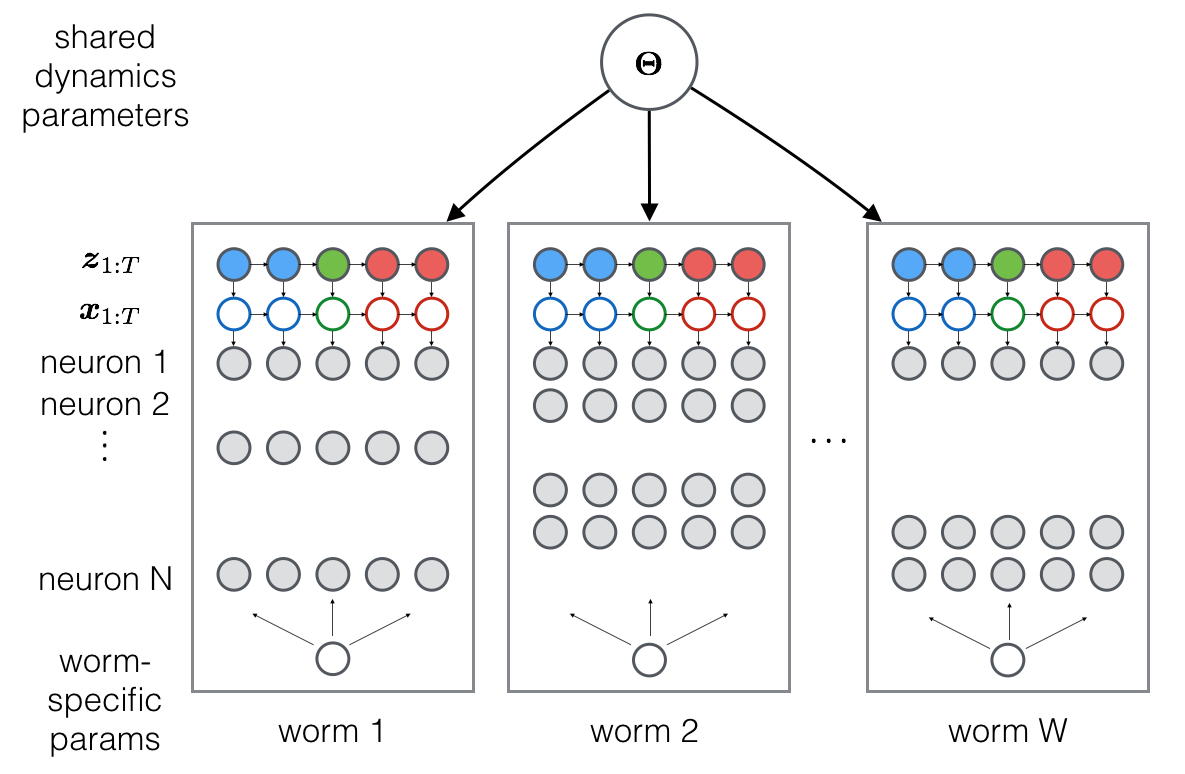
\includegraphics[width=5.5in]{hslds.png} 
\caption{A schematic of the hierarchical SLDS for combining information
  across multiple worms in order to learn a shared dynamical system
  for \celegans.  We have a set of shared set of model parameters,~$\bTheta$,
  represented by the large node at the top of the graphical model. Each
  worm,~$w$ has its own set of discrete latent states (colored nodes)
  and continuous latent states (nodes with colored outlines) and observed neurons.
  For example, neuron 1 may appear in all neurons whereas neuron 2
  may only be seen in worm 2. Thus, each worm provides information
  about the mapping from latent states to observations for only a
  subset of neurons. In terms of the model, this corresponds to a
  subset of rows in the matrix~$\bC$ and the vector~$\bd$. Finally,
  we allow each worm to have local parameters that capture, for example,
  the amount of fluorescent protein expressed in a particular neuron
  for a given worm. 
}
\label{fig:hslds}
\end{figure}

We propose the following hierarchical SLDS (hSLDS) to combine data from
multiple worms. Since these worms are genetically identical, we hypothesize
that their dynamics should be the same. That is, they share the same set
of~$K$ discrete states, as well as the
parameters~$\{\bA^{(k)}, \bb^{(k)}, \bQ^{(k)}, \bpi^{(k)}\}_{k=1}^K$.
We assume the following mapping from latent states to the neural activity
of worm~$w$, time~$t$, and neuron~$n$:
\begin{align}
  y_{w,t,n} &= \gamma_{w,n} (\bc_n^\trans \bx_{w,t} + d_{n}) + \epsilon_{w,t,n}, \\
  \epsilon_{w,t,n} &\sim \distNormal(0, r_{w,n}^2).
\end{align}
Thus, the mapping from latent states to the activity of neuron~$n$ is
partially shared across worms, in that all worms share the
vector~$\bc_n$.  These constitute the rows of an emission
matrix,~$\bC$. Note that, for simplicity, we have required all
discrete states,~$z_t$ to share the same emission matrix. However, we
have introduced a set of worm-specific, scalar
parameters,~$\{\gamma_{w,n}$ and~$r_{w,n}\}$. The
gain,~$\gamma_{w,n}$, captures differences in amplitude of the neural
signal that may arise from variation in fluorescent protein expression
from worm to worm.  The noise variance,~$r_{w,n}^2$, enables
neuron~$n$ to have different marginal variance from worm to worm,
which may arise due to a number of factors, like protein expression
levels and the clarity of a particular recording.  Whereas the general
SLDS allows for covariance in the noise from neuron to neuron, for
simplicity we have assumed that this matrix is worm-specific and
diagonal. Figure~\ref{fig:hslds} provides a graphical representation
of this model.

% Talk about the prior on gain... we used a truncated normal prior,
% maybe the fact that we needed such a constrained prior means that
% this gain parameter is a bad idea after all...

\section{Results}
\label{sec:results}
\begin{figure}[t]
\centering%
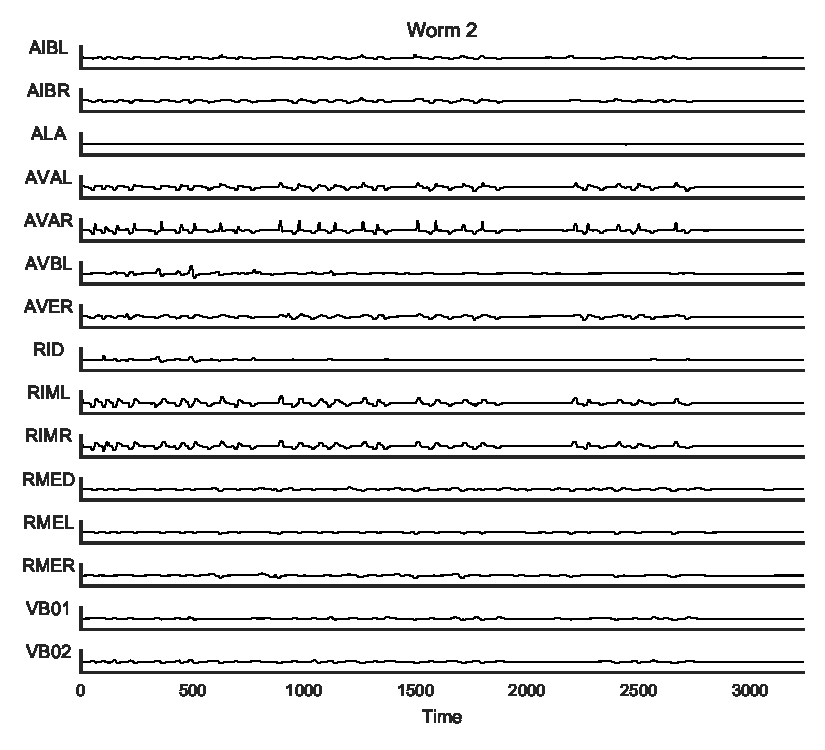
\includegraphics[width=5.5in]{shared_activity_worm1.pdf} 
\caption{Fluorescence traces of 15 neurons in the second worm. These
  neurons were identified in all 5 worms. Axis limits are the same for
  all neurons. }
\label{fig:shared_activity}
\end{figure}

We fit the hSLDS to recordings of five \textit{C. Elegans} collected
by \cite{kato2015global}. Each recording is 18 minutes long with a
sampling frequency of 3Hz, yield 3240 time steps per worm.  The
recordings contain~$N_w=109$, $107$, $131$, $126$, and $129$ neurons,
respectively. Of these, a subset have been manually identified.
Figure~\ref{fig:identified_neurons} shows the neurons that were
identified in each worm. We will capitalize on those neurons that are
identified in multiple worms in order to learn a shared subspace of
neural activity and a shared set of dynamical states for all
\textit{C. Elegans}. Figure~\ref{fig:shared_activity} shows the neural
activity of 15 identified neurons in the second worm. We immediately
recognize repeating patterns of activity; these will correspond to
characteristic ``loops'' in the low dimensional portrait of the
population activity.



\paragraph{Neural Activity is Low Dimensional}

% PCA trajectories of neural activity
\begin{figure}[t]
  \centering%
  \begin{subfigure}[b]{.19\linewidth}
    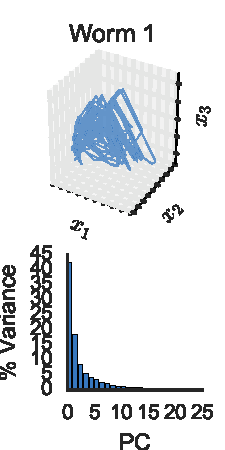
\includegraphics[width=\textwidth]{pca_trajectory_worm0.pdf}
  \end{subfigure}
  \begin{subfigure}[b]{.19\linewidth}
    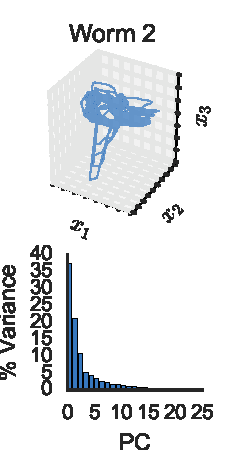
\includegraphics[width=\textwidth]{pca_trajectory_worm1.pdf}
  \end{subfigure}
  \begin{subfigure}[b]{.19\linewidth}
    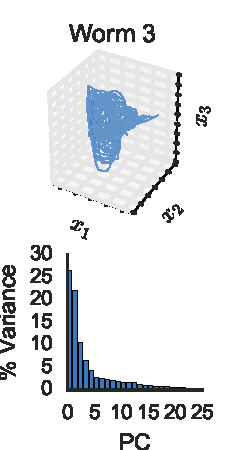
\includegraphics[width=\textwidth]{pca_trajectory_worm2.pdf}
  \end{subfigure}
  \begin{subfigure}[b]{.19\linewidth}
    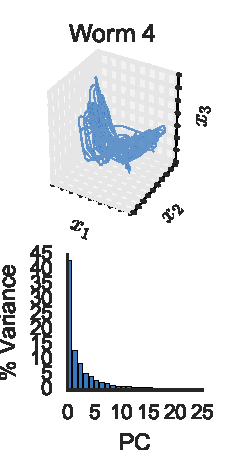
\includegraphics[width=\textwidth]{pca_trajectory_worm3.pdf}
  \end{subfigure}
  \begin{subfigure}[b]{.19\linewidth}
    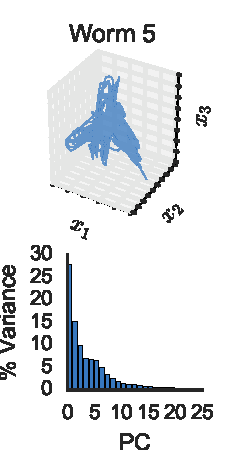
\includegraphics[width=\textwidth]{pca_trajectory_worm4.pdf}
  \end{subfigure} 
  \caption{Principal components analysis of each individual worm.
    In all cases, the neural activity is relatively low dimensional,
    with large percentages of the variance captured by the first three
    principal components (PC's). Above, the projection of roughly 100-dimensional
    neural activity onto the subspace spanned by the first three PC's.
    The hierarchical SLDS will find a common subspace for all worms, and,
    furthermore, segment the low dimensional trajectories into a sequence
    of discrete pieces.}
\label{fig:pca_trajectory}
\end{figure}

A fundamental assumption of the hSLDS is that neural activity is
low dimensional. To test this assumption, we first run principal
components analysis (PCA) on each worm's
population activity (a~$T \times N_w$ matrix) separately. We find
that the top three principal components (PC's)capture a large fraction
of the variance for all worms, as shown in the bottom panels of
Figure~\ref{fig:pca_trajectory}. The top panels show the projection
of neural activity onto the first three PC's. While the PCA
projections show qualitatively similar patterns, like intersecting
and orthogonal loops, the subspaces are not aligned across worms
and the trajectories are not particularly smooth or interpretable.
The hSLDS addresses these issues by learning a shared subspace
across all worms, and segmenting the low dimensional
trajectories into a sequence of states with simple, linear dynamics.


\paragraph{The hSLDS reveals a shared subspace and canonical dynamics across worms}

% Inferred dynamical system -- set of discrete latent states
\begin{figure}[t]
  \centering%
  \begin{subfigure}[b]{0.32\linewidth}
    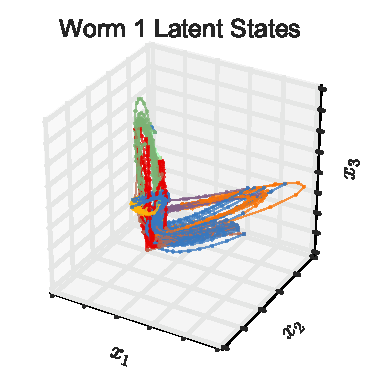
\includegraphics[width=\textwidth]{xs_3d_worm0.pdf}
  \end{subfigure}
  \begin{subfigure}[b]{0.32\linewidth}
    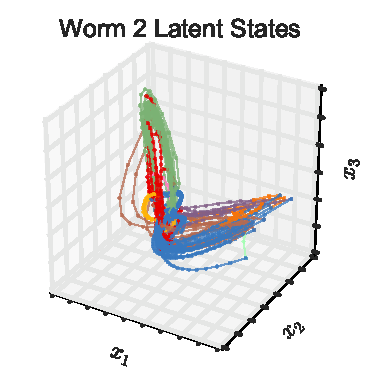
\includegraphics[width=\textwidth]{xs_3d_worm1.pdf}
  \end{subfigure}
  \\
  \begin{subfigure}[b]{0.32\linewidth}
    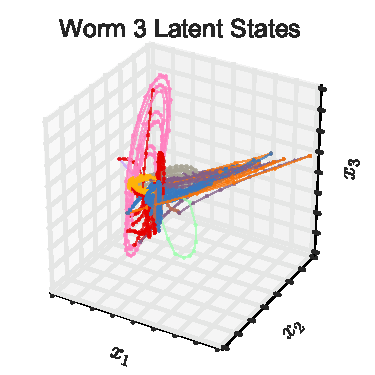
\includegraphics[width=\textwidth]{xs_3d_worm2.pdf}
  \end{subfigure}
  \begin{subfigure}[b]{0.32\linewidth}
    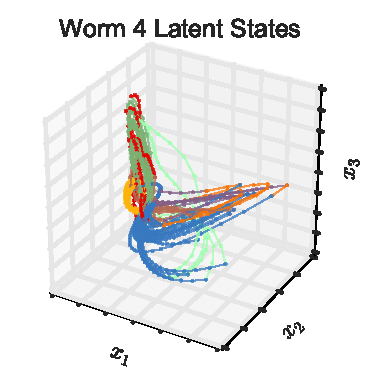
\includegraphics[width=\textwidth]{xs_3d_worm3.pdf}
  \end{subfigure}  
  \begin{subfigure}[b]{0.32\linewidth}
    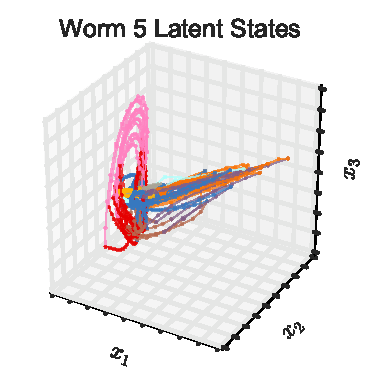
\includegraphics[width=\textwidth]{xs_3d_worm4.pdf}
  \end{subfigure}
  \caption{Latent states discovered by the hierarchical SLDS.
    Since the emission matrix,~$\bC$, is shared across worms, the
    coordinates of the latent states are shared as well. This
    reveals a common pattern of low dimensional activity characterized
    by interlocking and opposing loops. Colors denote the discrete
    latent state inferred for each part of the trajectory. For example,
    one loop begins with the latent state shooting out from the origin
    along the orange and purple states, and then returning via the blue
    state. Another begins with the green state, which swings upward and
    is then followed by a return via the red state. In worms 3 and 5,
    the upward swing is slightly tilted, as captured by the pink 
    rather than the green state. While harder to see in this view, there
    is a third loop in yellow that lies in the~$(x_1, x_2)$ plane.
    See supplementary videos for further detail.
  }
\label{fig:hslds_trajectory}
\end{figure}

The hSLDS shares information across worms in order to learn a
canonical subspace of neural activity and a common set of
low-dimensional dynamics. Figure~\ref{fig:hslds_trajectory} shows the
inferred continuous latent states,~$\bx_{1:T}$, of the hSLDS for each
of the five worms. There are three points to note, First, in contrast
to the PCA trajectories in Figure~\ref{fig:pca_trajectory}, the
similarity in hSLDS trajectories is readily apparent. This is due to
the fact that all worms share the same subspace, which is defined by the
global emission matrix~$\bC$. Second, the hSLDS trajectories
are considerably smoother than their PCA counterparts. This is a
direct result of the set of linear dynamics that comprise the hSLDS.
Assuming that the latent state,~$\bx_{t+1}$, is linearly related to the
preceding state,~$\bx_t$, induces an inductive bias toward smooth
trajectories in latent space. This reduces the discontinuities and noise
in the PCA trajectories and reveals the characteristic patterns of
latent dynamics. Third, the hSLDS trajectories have been segmented into
snippets, each corresponding to a different discrete latent state,~$z_t$, with
its own set of linear dynamics. These discrete states illustrated
as different colors in the hSLDS trajectories. These provide a
handle into understanding the latent dynamics of \textit{C. Elegans}
population activity, and a useful latent variable for relating
activity to behavior.

\paragraph{Neural dynamics switch between a set of linear regimes}
% 3D dynamics
\begin{figure}[th!]
  \centering%
  \begin{subfigure}[b]{0.32\linewidth}
    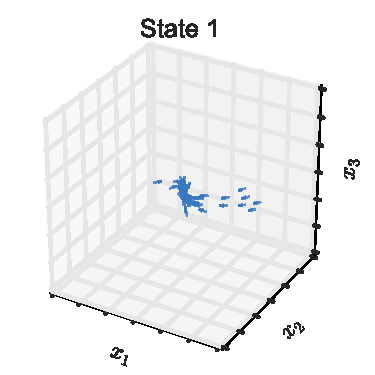
\includegraphics[width=\textwidth]{dynamics_3d_0.pdf}
  \end{subfigure}
  \begin{subfigure}[b]{0.32\linewidth}
    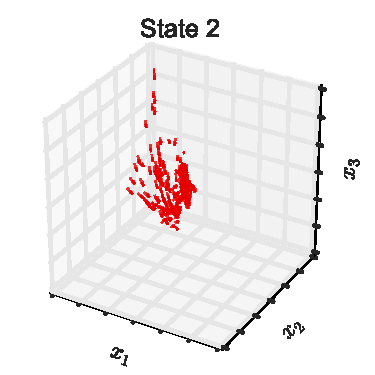
\includegraphics[width=\textwidth]{dynamics_3d_1.pdf}
  \end{subfigure}
  \begin{subfigure}[b]{0.32\linewidth}
    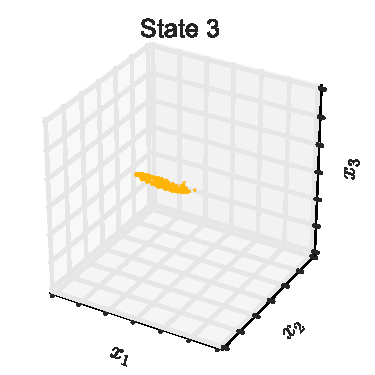
\includegraphics[width=\textwidth]{dynamics_3d_2.pdf}
  \end{subfigure}
  \\
  \begin{subfigure}[b]{0.32\linewidth}
    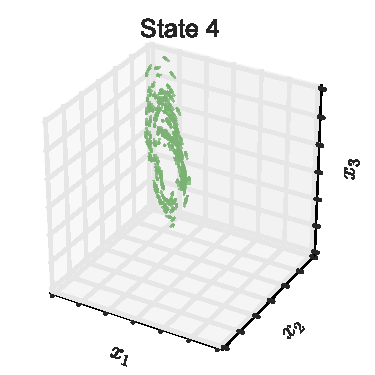
\includegraphics[width=\textwidth]{dynamics_3d_3.pdf}
  \end{subfigure}
  \begin{subfigure}[b]{0.32\linewidth}
    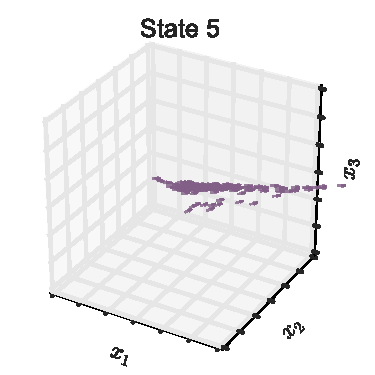
\includegraphics[width=\textwidth]{dynamics_3d_4.pdf}
  \end{subfigure}
  \begin{subfigure}[b]{0.32\linewidth}
    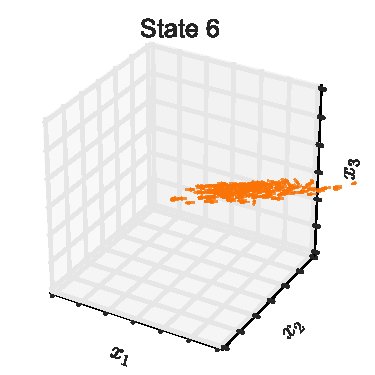
\includegraphics[width=\textwidth]{dynamics_3d_5.pdf}
  \end{subfigure}
  \\
  \begin{subfigure}[b]{0.32\linewidth}
    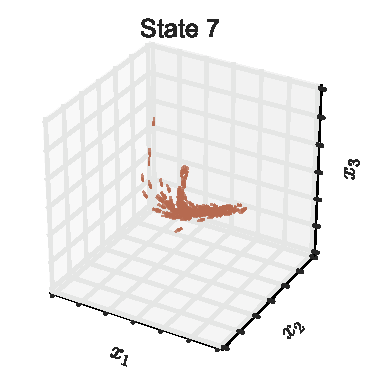
\includegraphics[width=\textwidth]{dynamics_3d_6.pdf}
  \end{subfigure}
  \begin{subfigure}[b]{0.32\linewidth}
    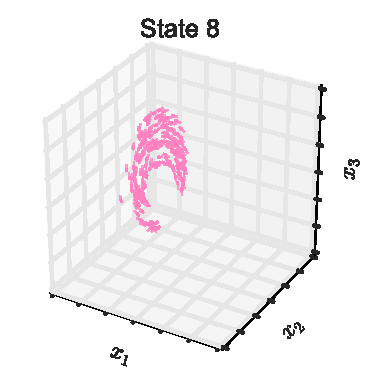
\includegraphics[width=\textwidth]{dynamics_3d_7.pdf}
  \end{subfigure}
  \begin{subfigure}[b]{0.32\linewidth}
    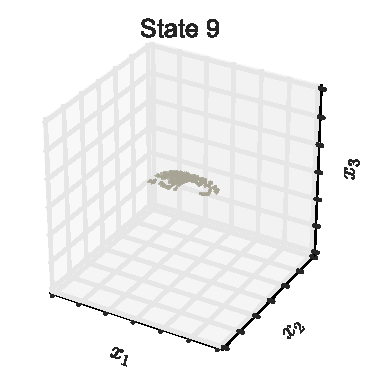
\includegraphics[width=\textwidth]{dynamics_3d_8.pdf}
  \end{subfigure}  
%  \\
%  \begin{subfigure}[b]{0.32\linewidth}
%    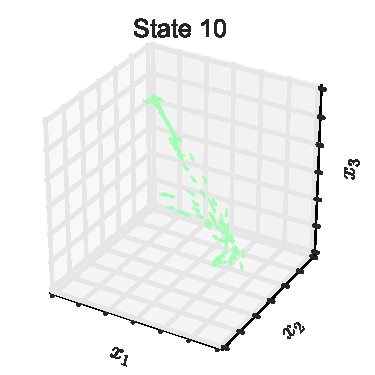
\includegraphics[width=\textwidth]{dynamics_3d_9.pdf}
%  \end{subfigure}
%  \begin{subfigure}[b]{0.32\linewidth}
%    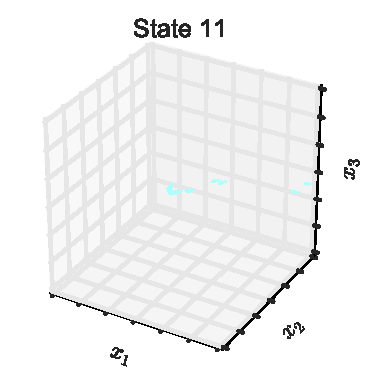
\includegraphics[width=\textwidth]{dynamics_3d_10.pdf}
%  \end{subfigure}
%  \begin{subfigure}[b]{0.32\linewidth}
%    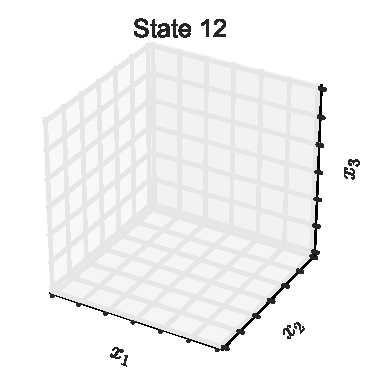
\includegraphics[width=\textwidth]{dynamics_3d_11.pdf}
%  \end{subfigure}  
  \caption{The discrete dynamical states that compose this switching
    linear dynamical system. The vector fields point in the direction of
    ~$\bA^{(k)} \bx + \bb^{(k)}$~($k=1 \ldots 9$). While the dynamics are
    defined for all~$\bx$,
    they are only plotted at locations where the corresponding state is used.
    States are ordered from most common (1)
    to least common (9); see supplementary material for remainder of
    states. The most common states (1 and 2) simply decay to the
    origin. State 3 is a tight loop in the~$(x_1, x_2)$ plane. States
    4 and 8 are larger loops in the~$(x_2, x_3)$ plane. States 5, 6,
    and 9 are sections of a third loop opposite to State 3. Finally,
    State 7 seems to bridge between loops.}
\label{fig:dynamics}
\end{figure}

As we have stated, the hSLDS segments the low dimensional trajectories
into a sequence of discrete states, each governed by simple linear dynamics.
These dynamics are shown in Figure~\ref{fig:dynamics}. The states are ordered
from most common (State 1) to least common (State 9). The model was fit with~$K=15$
states, but only 11 were used. The remaining two are omitted from this figure
since they are used very rarely. The vector fields shown here point in the
direction of~$\bA^{(k)} \bx_t + \bb^{(k)}$ for~$k=1, \ldots, 9$. While these
dynamics are defined for all~$\bx_t \in \reals^3$, for clarity, they are only plotted
at the locations in latent space where the corresponding state is deployed.

The most common states (1 and 2) correspond to decays toward the origin.
This is to be expected, since the neurons are quiescent most of the time
(c.f. Figure~\ref{fig:shared_activity}). The remaining states capture
different sections of the intersecting loops seen in Figure~\ref{fig:hslds_trajectory}.
State 3 is a short loop to the left in the~$(x_1, x_2)$ plane. States 4
and 8 correspond to the large upward swings that trace out loops in the~$(x_2, x_3)$
plane. States 5, 6, and 9 correspond to loops that swing out to the right
of the origin, again in the~$(x_1, x_2)$ plane. Finally, state 7 seems to
connect the~$(x_2, x_3)$ loop to the~$(x_1, x_2)$ loop, bypassing the origin.

This discrete segmentation of the latent state trajectories serves multiple
purposes. First, by stitching together discrete states with unique
linear dynamics, the hSLDS models a globally \emph{nonlinear} dynamical
system.  Second, these discrete latent states provide a valuable covariate
for understanding switches in the neural activity. As we will see below,
when we condition on the entry into these discrete states, characteristic
patterns of population activity are revealed. Third, these states provide
an interpretable summary of the complex, global brain activity. Next, we
will show that these discrete states correspond to meaningful behaviors.

\paragraph{Discrete states correspond to distinct behaviors}

% Discrete state transitions mimic those of hand-labeled behavioral segments
\begin{figure}[t]
\centering%
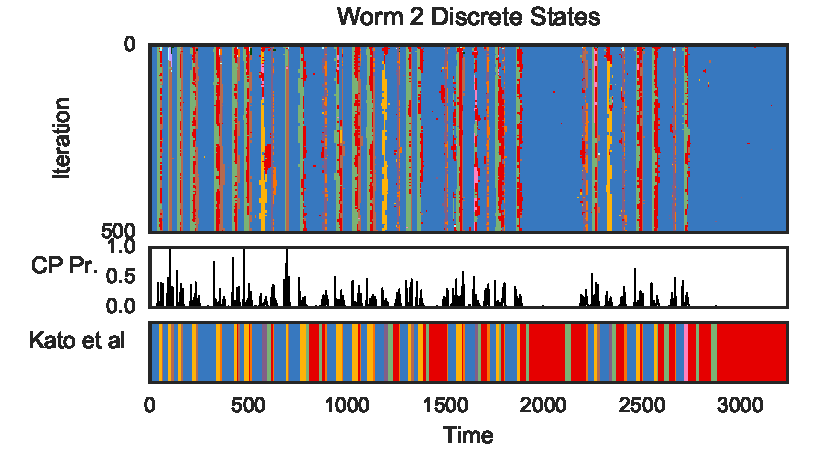
\includegraphics[width=5.5in]{discrete_state_cps_worm1.pdf} 
\caption{The inferred discrete states align with the manual segmentation
  of \citet{kato2015global}. \textit{Top:} samples from the posterior
  distribution of discrete states,~$z_{1:T}$. Each row is a sample, and
  each color denotes a distinct value from 1 to~$K=15$. \textit{Middle:}
  from these samples we estimate the probability of a change-point
  (i.e.~$z_t \neq z_{t-1}$). \textit{Bottom:} The inferred change-points
  align with the manual segmentation of \citet{kato2015global}. Note,
  however, that the colors do not perfectly align since there is not a
  one-to-one correspondence between the inferred and manual states. For
  example, the blue and red states of~\citet{kato2015global}, which
  correspond to ``REVSUS'' and ``SLOW,'' respectively, are combined into
  inferred State 1.
}
\label{fig:discrete_state_comparison}
\end{figure}

\citet{kato2015global} manually labeled segments of time corresponding to
distinct behaviors, like forward or reverse crawling and dorsal or ventral
turns. This process is both laborious and subjective. The hSLDS provides
a principled and automated alternative to manual labeling, by automatically
segmenting activity into snippets governed by linear dynamics. We find that
the manual and hSLDS segmentations are closely aligned.

Figure~\ref{fig:discrete_state_comparison} illustrates both the uncertainty
of the discrete labeling as well as the alignment with the ``ground truth''
labels. The top panel shows samples from the posterior distribution over
latent state sequences. Each row corresponds to a sample of~$z_{1:T}$, and
as before, the colors denote different discrete states. The variability
from sample to sample highlights the uncertainty that is inherent in assigning
a discrete label to a point in time --- where one state ends and the next
begins is not entirely clear from the noisy data.

From this sequence of discrete state samples we derive an estimate of the
\emph{change-point probability}, i.e. the probability that~$z_t \neq z_{t-1}$.
This is shown in the middle panel. In some instants it is eminently clear
that the discrete state has switched; this is due to large changes in the
dynamical trajectory that favor one state over another. More often, however,
this probability is lower and distributed over a window of time. Thus, our
Bayesian approach provides a principled means of assessing this uncertainty.

% Neural reconstruction
\begin{figure}[t]
\centering%
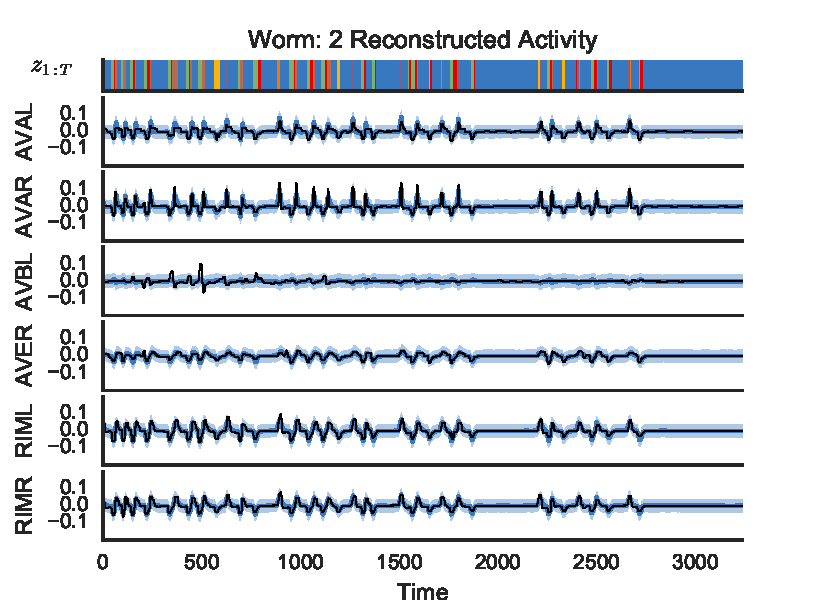
\includegraphics[width=5.5in]{neural_activity_worm_1.pdf} 
\caption{Observed (black) and smoothed (blue) activity of six neurons
  from worm 2. The smoothed activity is given by~$\gamma_{w,n}
  (\bc_n^\trans \bbE[\bx_{w,t}] + d_n)$. Shading denotes ~$\pm 1$
  standard deviation under the posterior given by~$\sqrt{\gamma_{w,n}^2 \bc_n^\trans
    \text{Var}[\bx_{w,t}] \bc_n + \sigma^2_{w,n}}$. Inferred discrete states
  are shown above for reference. }
\label{fig:neural_reconstruction}
\end{figure}


Finally, we see that these change-points align with the manual segmentation
of~\citet{kato2015global}, which is shown in the bottom panel. Note that the
manual and inferred state labels are not in one-to-one correspondence. This
is to be expected given both the invariance to permutation (though both are
sorted by usage), but more importantly because some manual states are grouped
into one inferred state. For example, the red and blue manual states, which
are labeled ``REVSUS'' and ``SLOW'', respectively, are combined in the blue
inferred state. Likewise, the manual sequence of purple followed by green,
which corresponds to a dorsal turn followed by a forward crawl, is combined
in the yellow inferred state.
Other states, like the yellow manual state, which corresponds
to a ventral turn, are separated into two inferred states, here red
and green. While the exact divisions between states are somewhat arbitrary,
the change points in these trajectories are clearly revealed by the hSLDS.


\paragraph{The hSLDS captures salient patterns of neural activity}

% Reconstruct the neural activity
As a generative model, the hSLDS provides a distribution over observed
neural activity. This provides a valuable sanity check for our results ---
does the model capture the variability of the data?
Figure~\ref{fig:neural_reconstruction} shows that indeed it does. We
plot the observed traces of six neurons in black and the predicted traces
under the posterior of the hSLDS in blue. With a Bayesian approach, we
also obtain an estimate of the uncertainty of these predictions, shown
here as shaded blue regions around the mean. We see that for most neurons,
the predicted and observed trajectories are well aligned, indicating that
the hSLDS with~$D=3$ dimensional latent states has sufficient capacity
to capture the variability of the data; however, some spikes in the activity
of neuron AVBL are smoothed over in this reconstruction. 

% Where do neurons lie in latent space?
% - which neurons are most interesting?
% - any listed in their paper
\paragraph{The hSLDS discovers a low-dimensional embedding of neurons}
\begin{figure}[t]
\centering%
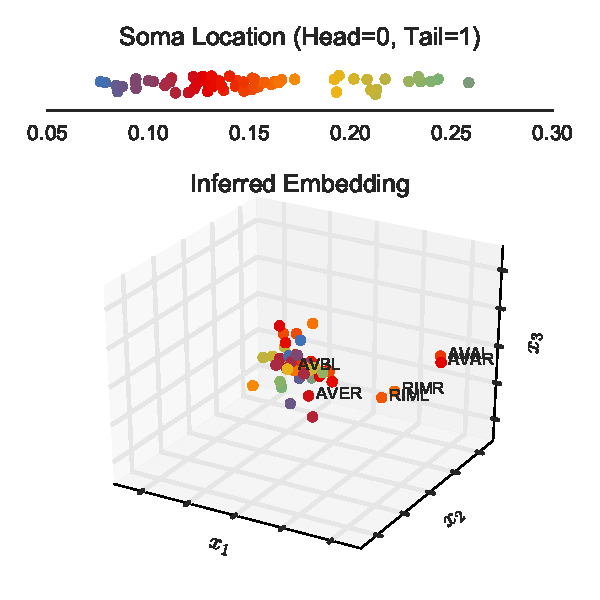
\includegraphics[width=4.in]{neuron_embedding.pdf} 
\caption{Three-dimensional embedding of neurons given by the
  rows of the emission matrix,~$\bc_n$. For reference, the
  true, one-dimensional location of the soma is shown above
  (jittered for clarity). While most neurons are clustered
  near the origin (reflecting the fact that most neurons
  have low amplitude activity), the more active neurons (shown
  above) stand out.}
\label{fig:neuron_embedding}
\end{figure}

In addition to yielding an interpretable, low-dimensional portrait
of neural activity, the hSLDS also provides an embedding of neurons
in latent space via the rows of the emission matrix,~$\bC$. Nearby
neurons in latent space will have highly correlated activity, and neurons
that are opposed will be anti-correlated. Figure~\ref{fig:neuron_embedding}
shows this embedding for the 60 neurons that are identified in at least
one of the five worms. For reference, the true one-dimensional location
of the neuron's soma along the head to tail axis is shown above.
Most of the neurons are clustered around the origin, reflecting the fact
that most neurons have little activity. However, two pairs of neurons
stand out: (AVAL, AVAR) and (RIML, RIMR). These pairs of neurons have larger
amplitude activity as shown above. These pairs both drive backward locomotion
(reversal), and are correlated via a gap junction.

% State entry triggered neural responses
\paragraph{Discrete state onset reveal stereotyped population activity}

\begin{figure}[t]
  \centering%
  \begin{subfigure}[b]{5.5in}
    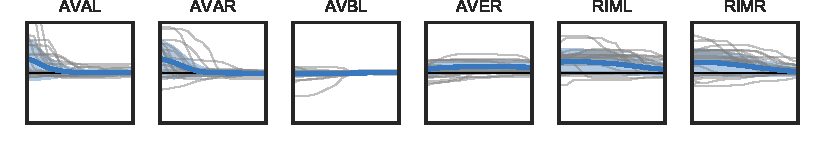
\includegraphics[width=\textwidth]{neural_responses_subset_0.pdf}
  \end{subfigure} \\
  \begin{subfigure}[b]{5.5in}
    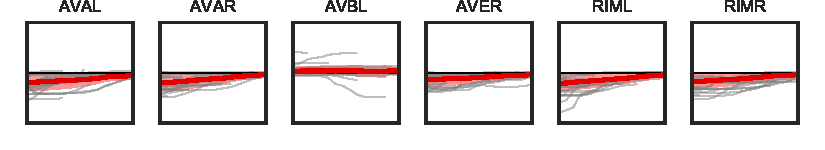
\includegraphics[width=\textwidth]{neural_responses_subset_1.pdf}
  \end{subfigure} \\
  \begin{subfigure}[b]{5.5in}
    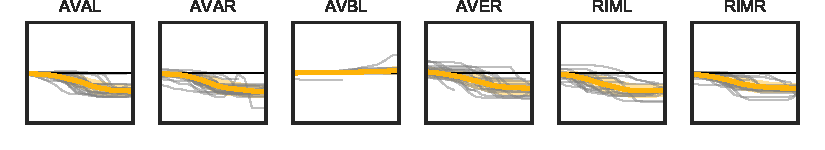
\includegraphics[width=\textwidth]{neural_responses_subset_2.pdf}
  \end{subfigure}\\
  \begin{subfigure}[b]{5.5in}
    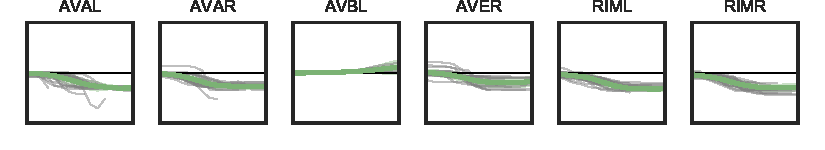
\includegraphics[width=\textwidth]{neural_responses_subset_3.pdf}
  \end{subfigure}
  \caption{Neural activity conditioned upon entry into each discrete
    state. The~$x$-axis is time since entering the discrete state
    (from 0 to 5 seconds), and the $y$-axis is the average neural
    response~$\pm 2$ standard deviations.  Light gray traces show a
    sample of individual neural activity traces.  Each row corresponds
    to the discrete state with the corresponding color. Here shown are
    States 1-4.}
  \label{fig:state_trigged_activity_1}
\end{figure}

\begin{figure}[t]
  \centering%
  \begin{subfigure}[b]{5.5in}
    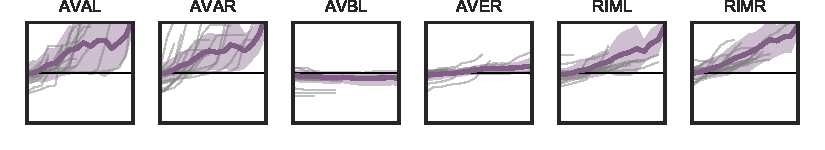
\includegraphics[width=\textwidth]{neural_responses_subset_4.pdf}
  \end{subfigure} \\
  \begin{subfigure}[b]{5.5in}
    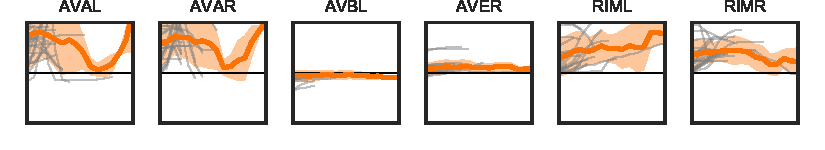
\includegraphics[width=\textwidth]{neural_responses_subset_5.pdf}
  \end{subfigure} \\
  \begin{subfigure}[b]{5.5in}
    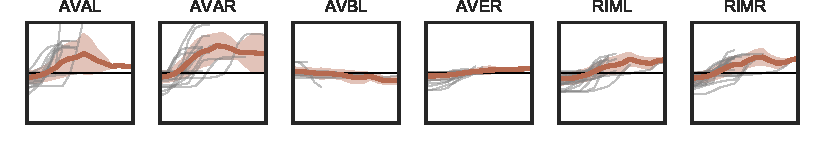
\includegraphics[width=\textwidth]{neural_responses_subset_6.pdf}
  \end{subfigure}\\
  \begin{subfigure}[b]{5.5in}
    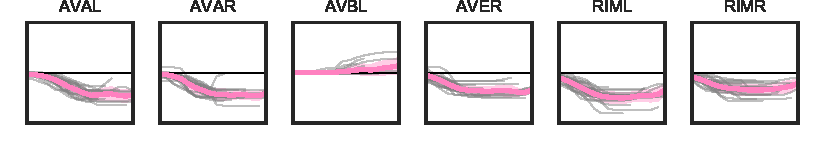
\includegraphics[width=\textwidth]{neural_responses_subset_7.pdf}
  \end{subfigure}
  \caption{Same as figure above but for States 5-8.}
  \label{fig:state_trigged_activity_2}
\end{figure}

The discrete latent states partition neural activity into interpretable
and behaviorally relevant segments. As such, they are natural covariates
for neural activity. Figures~\ref{fig:state_trigged_activity_1}
and~\ref{fig:state_trigged_activity_2} illustrate the distribution of
neural responses upon entry into each of the top 8 discrete states.
The~$x$ axis in these plots denotes time from 0 to 5
seconds after entry into the corresponding state. The colored line
denotes the mean response of the corresponding neuron (same $y$ limits
in all panels), and the shaded regions denote~$\pm 2$ standard deviations.
The light gray traces show a sample of randomly chosen neural responses.
That AVA and RIM neurons are associated with reverse crawling suggests
that states 2, 3, and 8 are related to forward locomotion (since the neural
activity is decreasing) and states 5, 6, and 7 are related to the
reverse locomotion (since the activity is increasing). 

% Residual analysis -- how well does the model fit?
% - baselines: probabilistic PCA, classical SLDS
% - note that these are less constrained!

\section{Discussion}
The elucidation of global brain dynamics and their relation to behavior
is perhaps the foremost goal of systems neuroscience. \celegans, with
its well-studied connectome and corresponding array of optical imaging tools,
provides many exciting opportunities to make progress toward this goal.
To do so, however, requires statistical methods capable of revealing latent
structure in complex neural data, and combining data across many worms.
The hierarchical SLDS satisfies many of these demands, decomposing
high-dimensional, nonlinear dynamics into a sequence of discrete latent
states with low-dimensional, linear dynamics. Moreover, by sharing across
worms while allowing for individual variability, the hSLDS reveals a
common set of latent dynamics.

% Remaining questions
Many questions remain. First, as a generative model, the hSLDS falls
somewhat short with its relatively limited model for discrete dynamics.
It is clear from these portraits of neural activity that discrete states
are deployed in very localized regions of latent space. Our recent work on
recurrent switching linear dynamical systems (rSLDS) leverages this type
of structure \citep{linderman2016recurrent}. In future work, we intend to
combine the hSLDS and rSLDS and apply them to this data.

Second, our analyses of state-triggered neural activity have only scratched
the surface. We intend to look more closely at the population responses
in these distinct latent states and search for further insights into how
this low-dimensional population activity drives behavior.

Third, we have not leveraged the availability of the \celegans connectome
in this work. In theory, this connectome should provide strong information
about the correlational structure of population activity. It remains an
open question how best to combine this anatomical data with state space
models like these.

Finally, while we have utilized the neurons that are found in multiple
worms to learn a shared subspace of activity and a common set of discrete
states, we could further improve upon this work by inferring neuron
identities for the hundreds of unlabeled neurons.  Their rough locations
and the correlations across worms provides a substantial amount of information
to tackle this problem.


\bibliographystyle{plainnat}
\bibliography{writeup}

\appendix

\section{Bayesian Inference for Switching Linear Dynamical Systems}
\label{app:mcmc}
Our goal is to estimate the posterior probability of a sequence 
of latent states and a set of parameters given the observed data.
From Bayes' rule, we have,
\begin{align}
  p(\bz_{1:T}, \bx_{1:T}, \bTheta \given \by_{1:T}) 
  &= 
  \frac{p(\by_{1:T}, \bx_{1:T}, \bz_{1:T}, \bTheta)}{p(\by_{1:T})}.
\end{align}
The numerator is the joint probability given by Eq.~\eqref{eq:joint}, and
the denominator,~$p(\by_{1:T})$, which is also known as the
\emph{marginal likelihood}, is given by an integral over possible
latent states and parameters,
\begin{align}
  p(\by_{1:T}) &= \int p(\by_{1:T}, \bx_{1:T}, \bz_{1:T}, \bTheta) 
  \, \mathrm{d}\bx_{1:T} \, \mathrm{d}\bz_{1:T} \, \mathrm{d}\bTheta.
\end{align}
Unfortunately, this integral is not efficiently computable for complex
models like the SLDS, forcing us to seek approximate inference methods
instead. Markov chain Monte Carlo (MCMC) methods \citep{gilks2005markov, robert2013monte} offer one
such approach. 

To construct our MCMC algorithm, we iteratively sample one set of 
latent states or parameters from its conditional distribution, holding 
the rest fixed, in a technique known as Gibbs sampling. 
There are five main sets of parameters to sample, detailed below.
\begin{enumerate}
  \item \textit{Gibbs sampling the discrete latent states,~$\bz_{1:T}$:}
    
    Given the continuous latent states,~$\bx_{1:T}$, and the
    parameters,~$\bTheta$, the conditional distribution over discrete
    latent states is the same as in a standard hidden Markov model. A
    joint sample from~$p(\bz_{1:T} \given \bx_{1:T}, \by_{1:T},
    \bTheta)$ can be generated using the forward filtering backward
    sampling (FFBS) algorithm.

  \item \textit{Gibbs sampling the continuous latent states,~$\bx_{1:T}$:}
    
    Given the discrete latent states,~$\bz_{1:T}$, the observations,~$\by_{1:T}$,
    and the parameters,~$\bTheta$, the conditional distribution of the 
    continuous latent states is linear and Gaussian. As with the discrete
    latent states, a joint sample of~$p(\bx_{1:T} \given \bz_{1:T}, \by_{1:T}, \bTheta)$
    can be generated using an FFBS algorithm.

  \item \textit{Gibbs sampling the dynamics parameters,~$\{\bA^{(k)}, \bb^{(k)}, \bQ^{(k)}\}_{k=1}^K$:}
    
    For fixed latent state sequences, the dynamics model reduces to a simple 
    multivariate regression problem. We have,
    \begin{multline}
      p(\bA^{(k)}, \bb^{(k)}, \bQ^{(k)}  \given \bz_{1:T}, \bx_{1:T}, \by_{1:T}, \bTheta)
      \\ 
      \propto
      p(\bA^{(k)}, \bb^{(k)}, \bQ^{(k)})
      \prod_{t=1}^T \left[ \,
        \distNormal(\bx_{t} \given \bA^{(k)} \bx_{t-1} + \bb^{(k)},\, \bQ^{(k)} \right]^{\bbI[z_{t-1}=k]}.
    \end{multline}
    If the prior distribution is the form of a matrix normal inverse Wishart (MNIW) prior, 
    then this conditional distribution will be as well. 

  \item \textit{Gibbs sampling the observation parameters,~$\{\bC^{(k)}, \bd^{(k)}, \bR^{(k)}\}_{k=1}^K$:}
    
    As with the dynamics parameters, 
    for fixed latent state sequences, the observation model is also a 
    multivariate regression problem. We have,
    \begin{multline}
      p(\bC^{(k)}, \bd^{(k)}, \bR^{(k)}  \given \bz_{1:T}, \bx_{1:T}, \by_{1:T}, \bTheta)
      \\ 
      \propto
      p(\bC^{(k)}, \bd^{(k)}, \bR^{(k)})
      \prod_{t=1}^T \left[ \,
        \distNormal(\by_{t} \given \bC^{(k)} \bx_{t} + \bd^{(k)},\, \bR^{(k)} \right]^{\bbI[z_{t}=k]}.
    \end{multline}
    This, too, is conjugate when the prior distribution assumes the
    form of a matrix normal inverse Wishart (MNIW) distribution.

  \item \textit{Gibbs sampling the Markov parameters,~$\{\bpi^{(k)}\}_{k=1}^K$:}
    
    Finally, we must sample the Markov transition matrix. We separate
    this into its~$K$ rows, each of which specifies a probability
    distribution,~$p(z_t \given z_{t-1}=k) = \bpi^{(k)}$.  For a fixed
    discrete latent state sequence, the conditional distribution of~$\bpi^{(k)}$ 
    is,
    \begin{align}
      p(\bpi^{(k)} \given \bz_{1:T}) &\propto
      p(\bpi^{(k)}) \prod_{t=1}^T \left[ \pi_{z_t}^{(k)} \right]^{\bbI[z_{t-1}=k]}.
    \end{align}
    If the prior distribution is~$p(\bpi^{(k)}) = \distDirichlet(\bpi^{(k)} \given \alpha)$, then this
    conditional distribution is a Dirichlet as well,
    \begin{align}
      p(\bpi^{(k)} \given \bz_{1:T}) 
      &= \distDirichlet(\bpi^{(k)} \given \widetilde{\balpha}^{(k)}) \\
      \widetilde{\alpha}_{k'}^{(k)} &= \alpha + \sum_{t=1}^T \bbI[z_t = k'] \, \bbI[z_{t-1}=k].
    \end{align}
\end{enumerate} 

Each one of these five steps leaves the desired posterior distribution as the 
unique stationary distribution of the Markov chain. Thus, by iterating these 
steps, the sampled states and parameters will eventually be distributed according
to their posterior probability given the observed data. Critically, the rate 
at which the Markov chain converges to its stationary distribution is determined
in part by the correlation between the sampled latent states at one iteration and
those at the next. If the chain only makes minor updates to the latent state sequence,
it will likely take a long time to converge to the desired posterior distribution.  
By performing joint, ``block'' updates of~$\bx_{1:T}$ and~$\bz_{1:T}$ in steps 
1 and 2, we find that the latent state sequences are able to be explored more 
efficiently.

\end{document}
